	\begin{Huge}
			Medizininformatik
		\end{Huge}
		\begin{exampleblock}{\textcolor{white}{Was ist der Studiengang?}}
			Die Schnittstelle zwischen Klinikum, Ärzten und Medizintechnikern. Klassische Anwendungsbereiche sind E-Health, Medizinische Datenverarbeitung sowie die (Mit-)Entwicklung von Medizingeräten. Es wird ein stärkerer Fokus auf Biologie, Physik und medizinische Inhalte gelegt. Ein Schwerpunktfach gibt es nicht.
		\end{exampleblock}
	
	\begin{block}{Welcher Teil macht wie viel im Studium aus?}
		\begin{figure}[h!]
			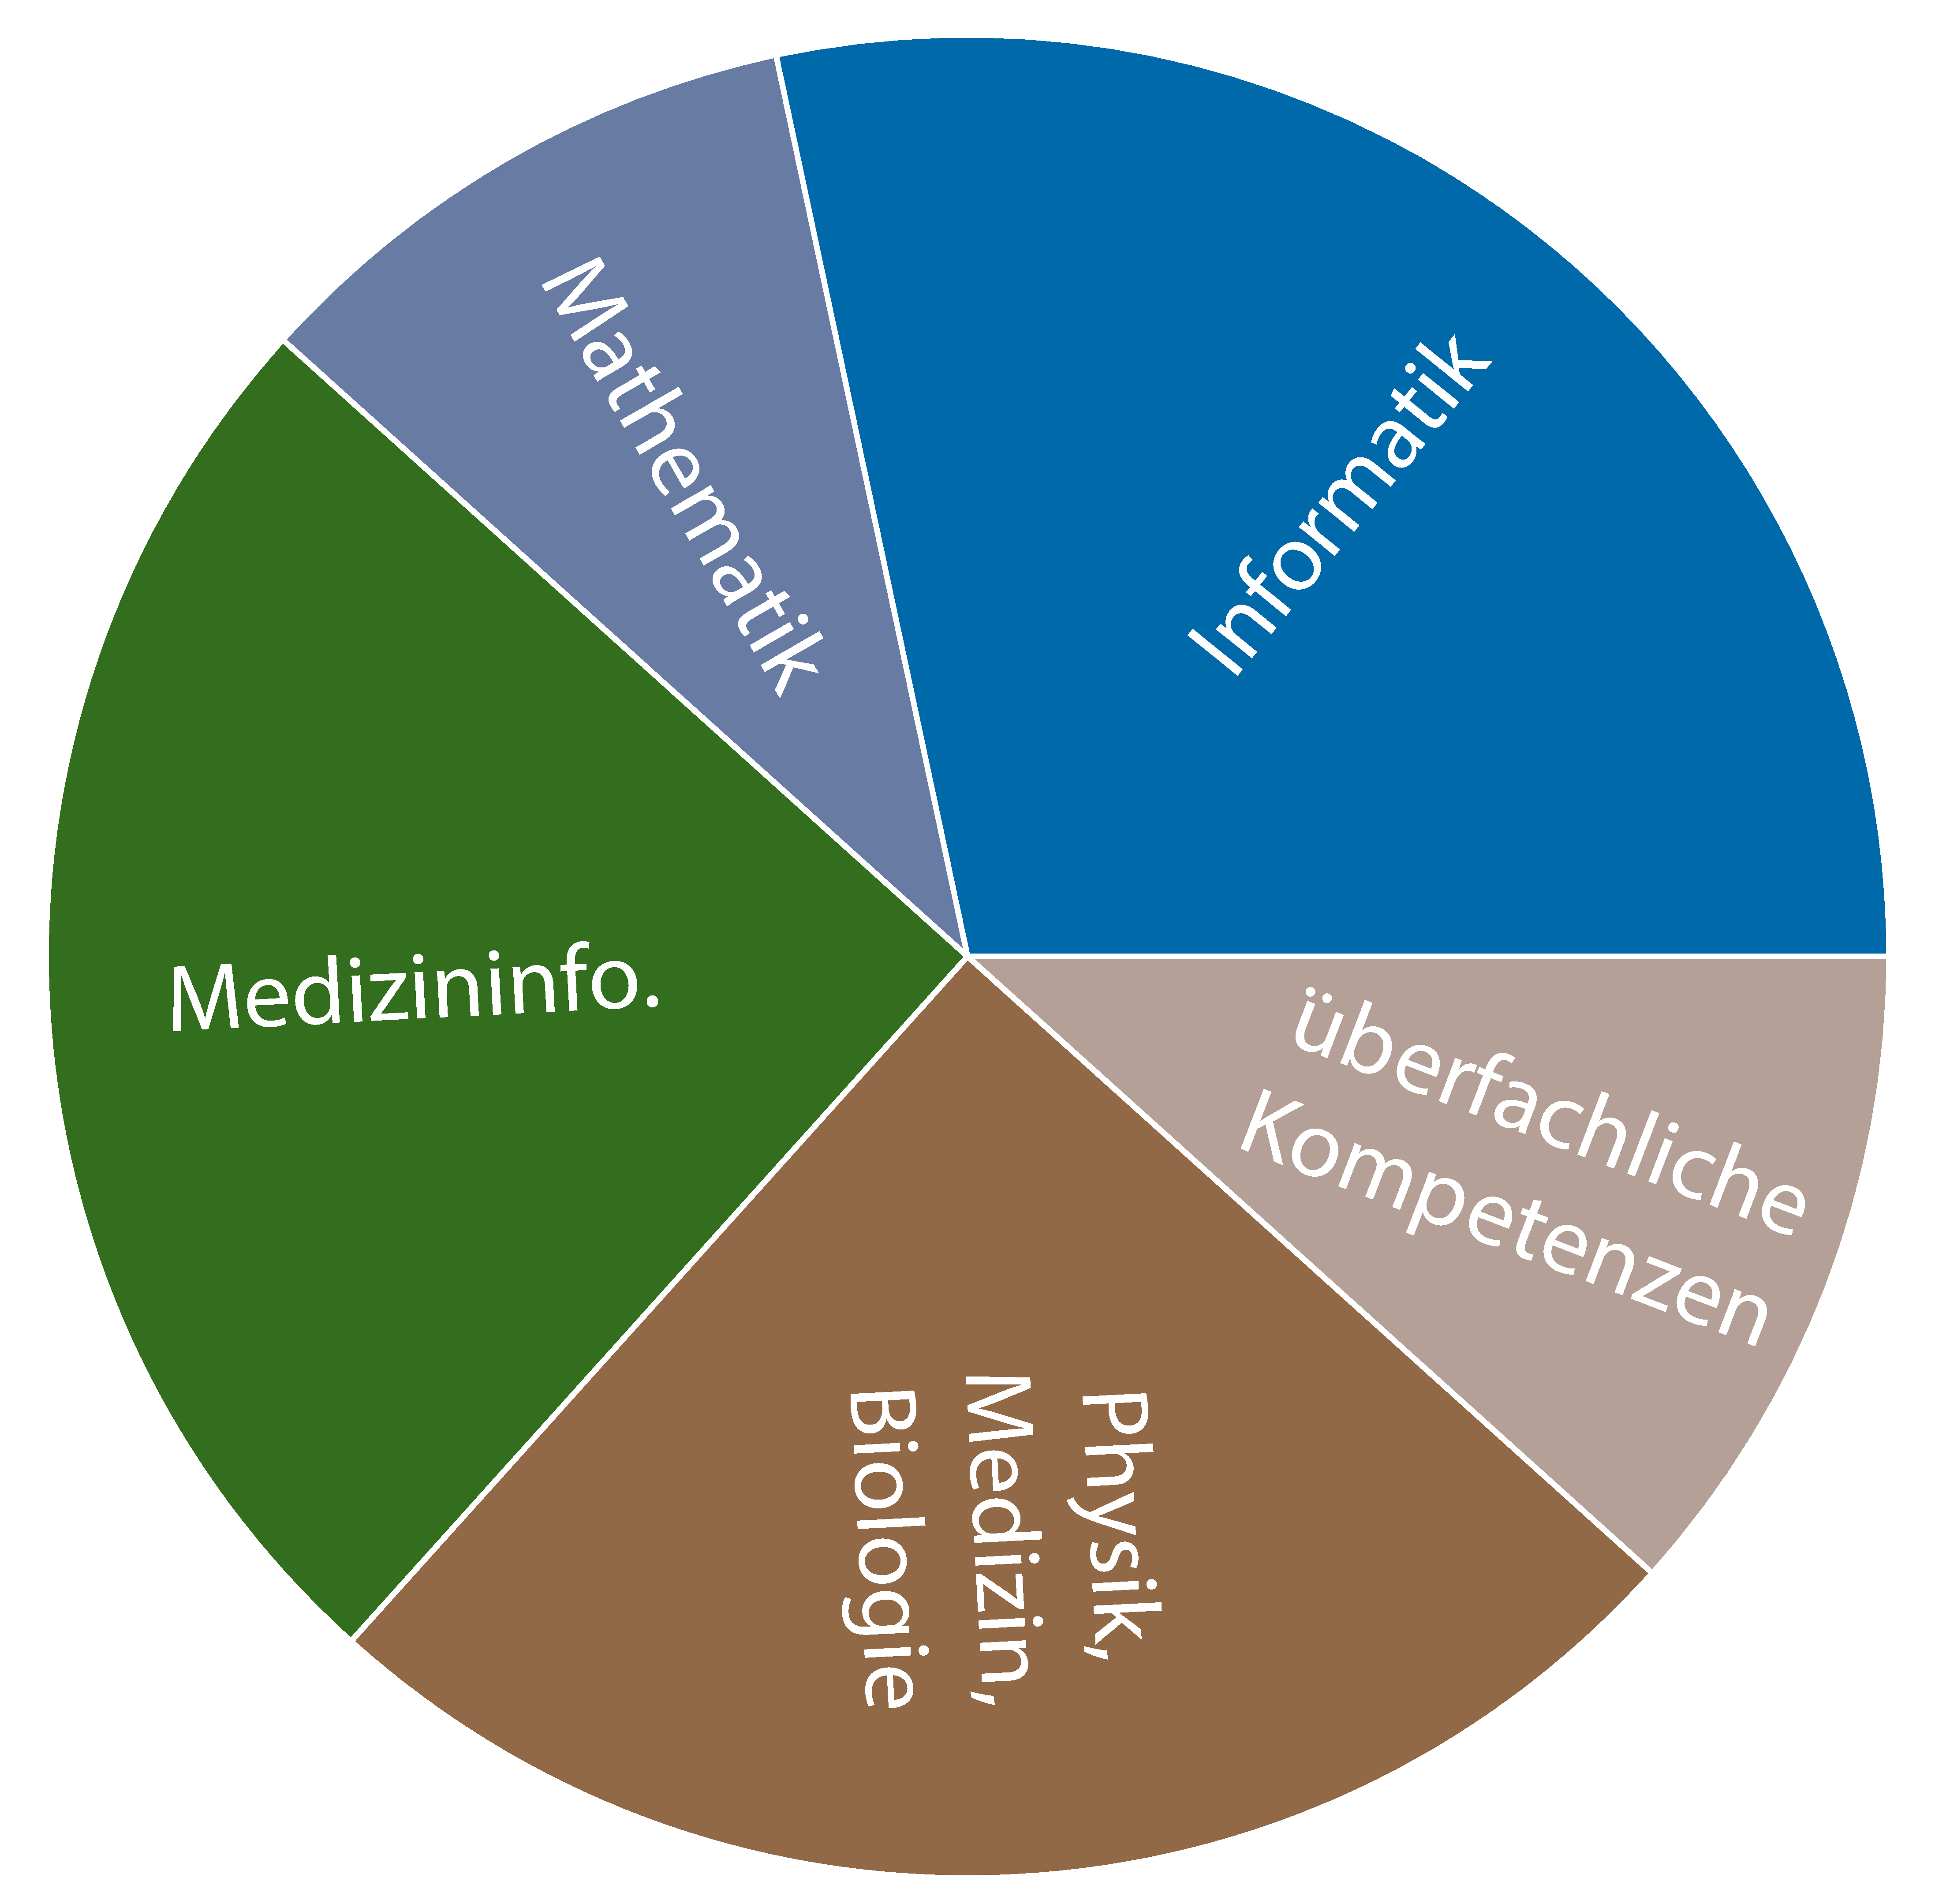
\includegraphics[width=0.4\textwidth]{charts/medizininformatik-Piechart.pdf}
			\caption{Verteilung der Themenbereiche über das komplette Studium}
		\end{figure}
	\end{block}
	
	\begin{block}{Was macht man in welchem Semester?}
		\begin{figure}[h!]
			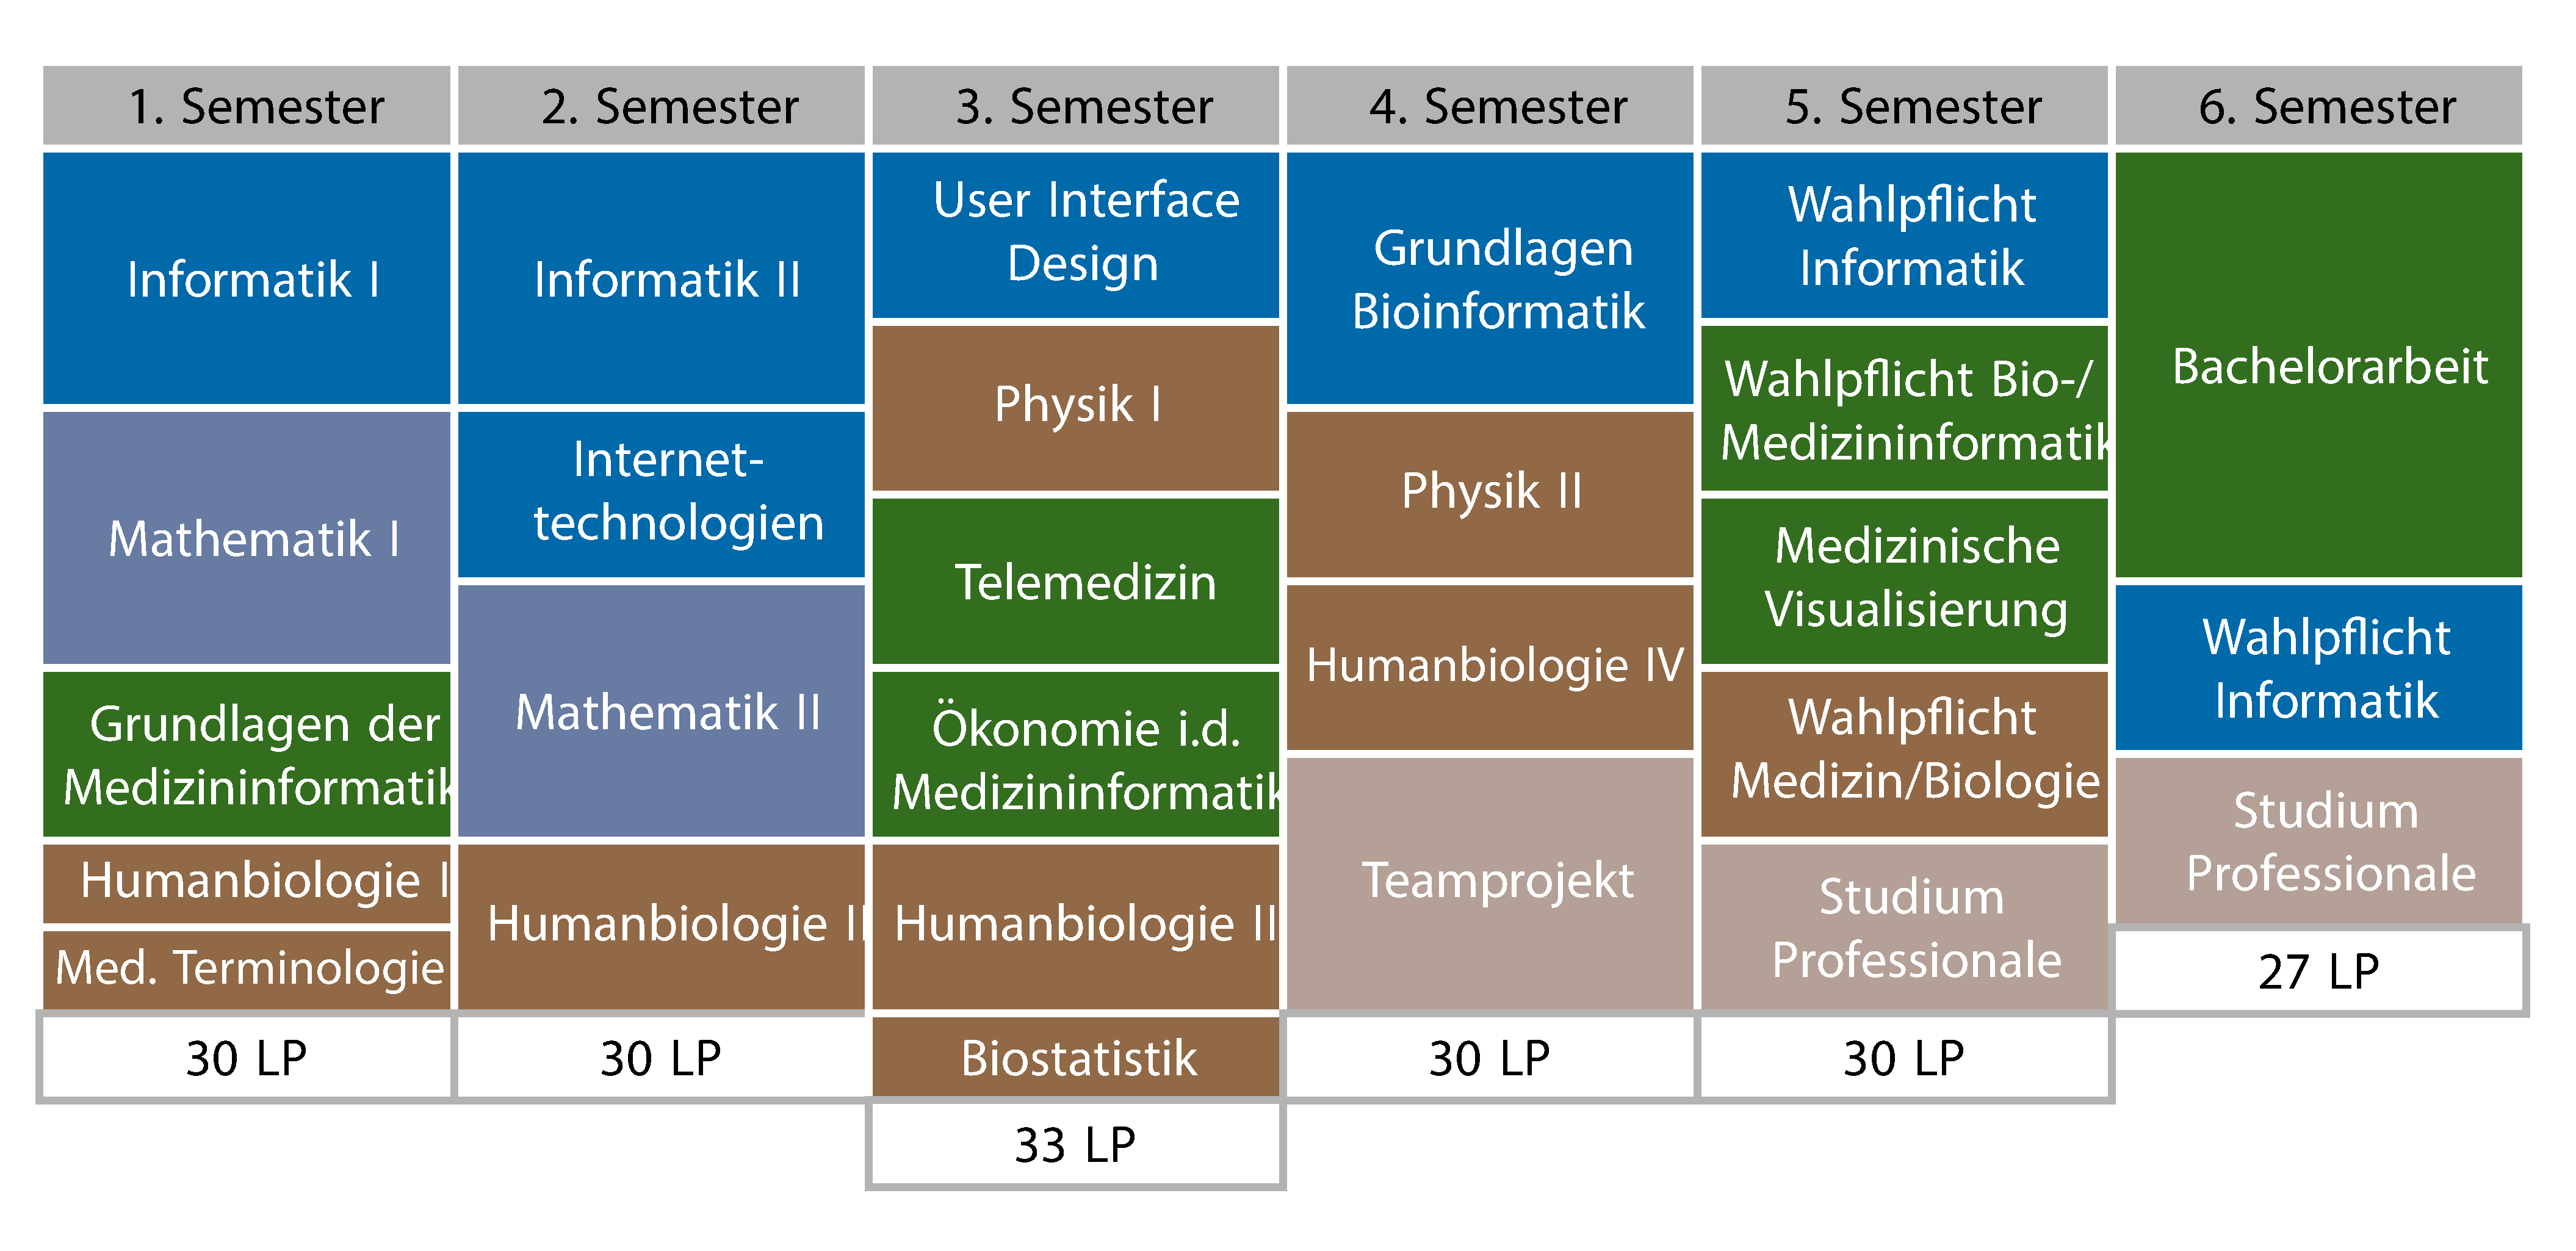
\includegraphics[width=\textwidth]{charts/medizininformatik_Studienplan_abWS18.pdf}
		\end{figure}
		Dieser Verlauf ist allerdings nur ein Vorschlag und kein bindender Studienplan. Es empfiehlt sich jedoch, den Plan einzuhalten, wenn man in Regelstudienzeit studieren möchte.
	\end{block}
